\documentclass[tikz,border=3.14mm]{standalone}
\usepackage{amsmath}
\usepackage{pgfplots}
\pgfplotsset{width=10cm, height=5cm,compat=1.9}
\begin{document}

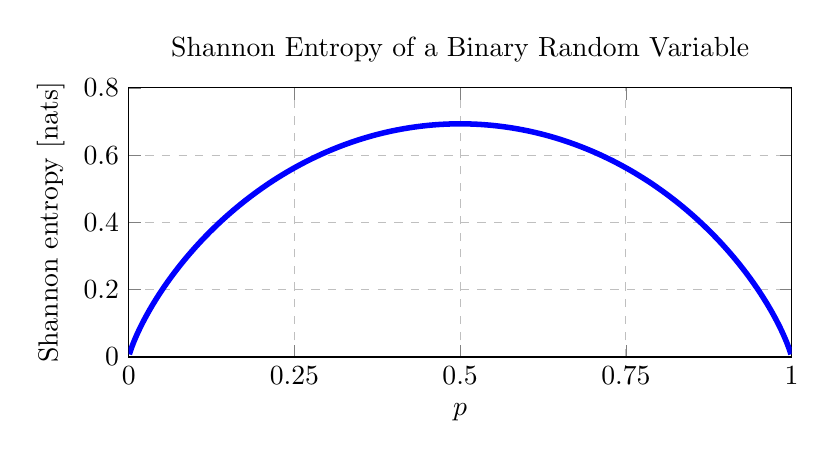
\begin{tikzpicture}
    \begin{axis}[
        title={Shannon Entropy of a Binary Random Variable},
        xlabel={$p$},
        ylabel={Shannon entropy [nats]},
        xmin=0, xmax=1,
        ymin=0, ymax=0.8,
        xtick={0,0.25, 0.5, 0.75, 1},
        ytick={0,0.2, 0.4, 0.6, 0.8},
        legend pos=north west,
        ymajorgrids=true,
        xmajorgrids=true,
        grid style=dashed,
    ]
    
    \addplot[
        domain=0.001:0.999, 
        samples=1000, 
        color=blue,
        line width=2pt
        ]
        {(x-1.0)*ln(1.0-x) - x*ln(x)};
        
    \end{axis}
    \end{tikzpicture}
\end{document}